\documentclass[notheorems, handout]{beamer}

\usetheme{Warsaw}
\setbeamertemplate{page number in head/foot}[totalframenumber]
\setbeamertemplate{headline}{}
\setbeamertemplate{navigation symbols}{}
\usefonttheme[onlymath]{serif}

\usepackage[utf8]{inputenc}
\usepackage[T2A]{fontenc}
\usepackage[russian]{babel}
\usepackage{graphicx,subcaption,ragged2e}
\usepackage{tikz}
\usepackage{bm}
\usepackage{physics}
\usepackage{amsmath,amsfonts,amssymb}
\usepackage{mathtools}

\newtheorem{theorem}{Теорема}

\title[Нейронные сети для изображений]{Свёрточные нейронные сети для обработки изображений: классификация и сегментация}

\institute[Санкт-Петербургский Государственный Университет]{%
  \small
  Санкт-Петербургский государственный университет\\
  Кафедра статистического моделирования
}
\date{28 октября 2025}
\newcommand{\vect}[1]{\mathbf{#1}}
\newcommand{\matr}[1]{\boldsymbol{#1}}

\begin{document}

\begin{frame}
    \titlepage
\end{frame}

\begin{frame}{Свёрточные нейронные сети (CNN)}
    \begin{itemize}
        \item Класс нейронных сетей, эффективно работающих с изображениями (и другими объектами, в которых важна пространственная связь);
        \item Используют свёртки (свёрточные слои) для извлечения признаков;
        \item Основные применения: классификация, сегментация, детекция объектов.
    \end{itemize}
    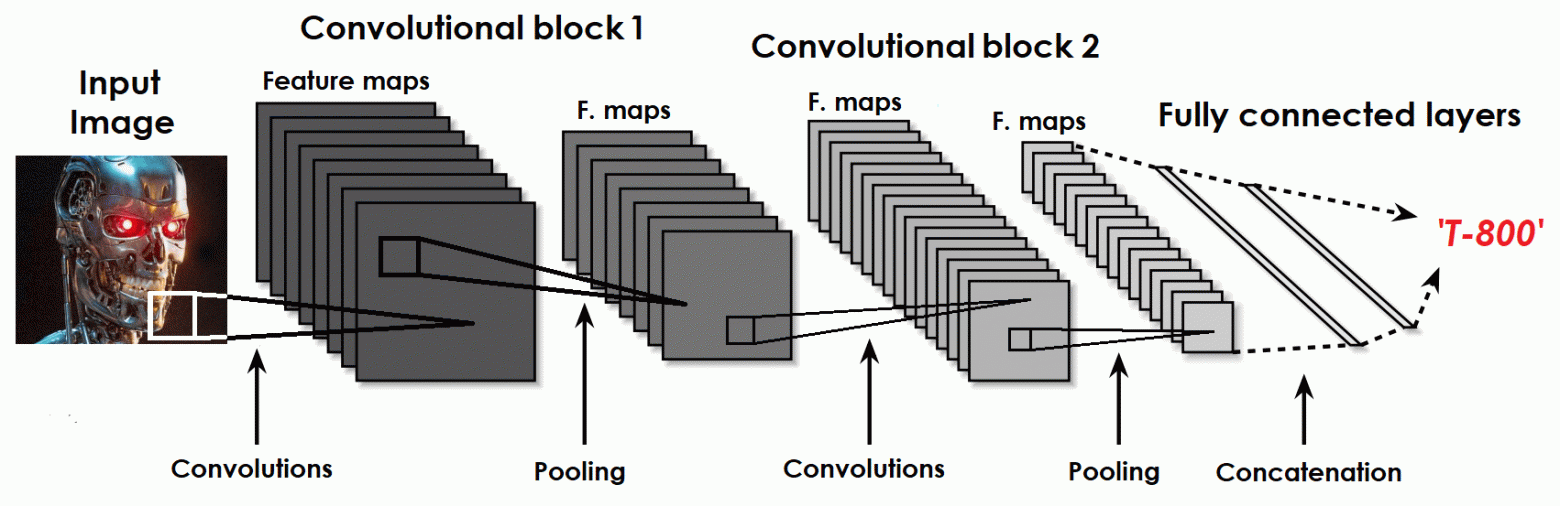
\includegraphics[width=\linewidth]{img/conv_nn.png}
\end{frame}

\begin{frame}{Проблемы обработки изображений полносвязными сетями}
    \begin{itemize}
        \item Изображения содержат пространственную структуру, которую теряют обычные полносвязные сети;
        \item Если изображение имеет высокое разрешение, то полносвязная сеть содержит слишком много параметров;
        \item При небольшом изменении изображения (сдвиг, поворот) входной слой обычной сети полностью меняется, хотя суть осталась прежней.
    \end{itemize}
    \begin{figure}
        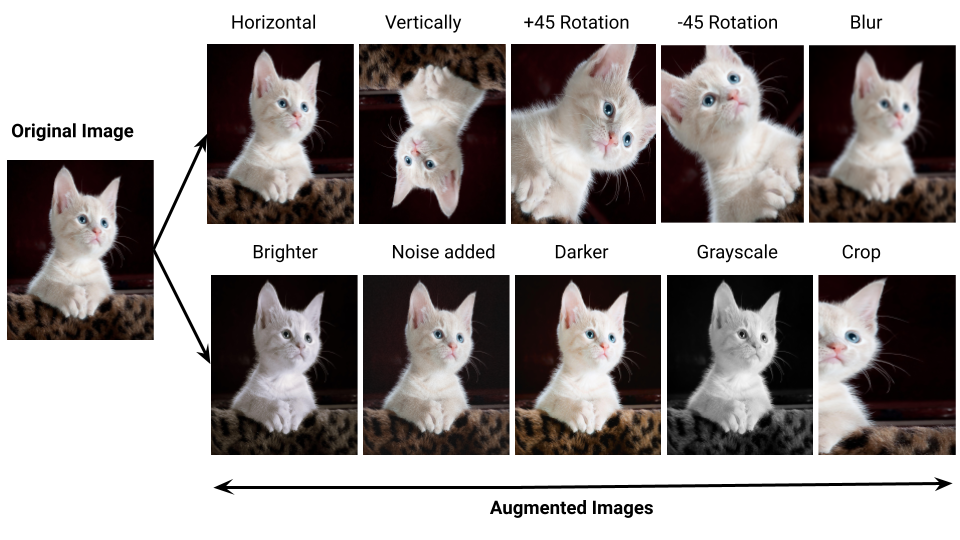
\includegraphics[width=0.7\linewidth]{img/augmentation.png}
    \end{figure}
\end{frame}

\begin{frame}{Основные компоненты CNN}
    \begin{figure}
        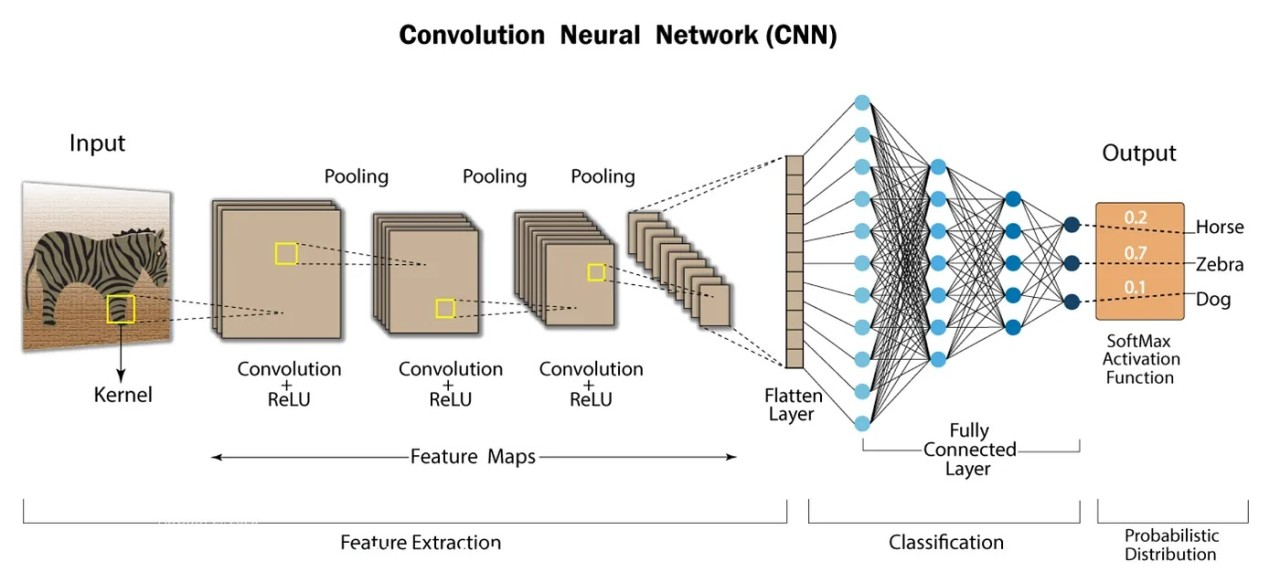
\includegraphics[width=0.8\linewidth]{img/conv_nn_layers.jpeg}    
    \end{figure}

    \begin{itemize}
        \item Свёрточные слои (Conv);
        \item Пулинг (Pooling, часто MaxPooling или AvgPooling);
        \item Нелинейности (ReLU, sigmoid, tanh и т.д.);
        \item Полносвязные слои.
    \end{itemize}

    С помощью свёрточных слоёв и пулинга изображение сводится до вектора размерности $1$, то есть формируется вход для полносвязной сети.
\end{frame}

\begin{frame}{Свёрточная операция}
    \begin{itemize}
        \item Свертка — это скользящее умножение ядра на участок изображения.
        \item Позволяет выделить локальные признаки (границы, текстуры).
    \end{itemize}

    % \[
    %     f _{i, j, c} = b _c + \sum _{p = 1} ^{C _{\text{in}}} \sum _{m = 0} ^{M - 1} \sum _{n = 0} ^{N - 1} W _{c, p, m, n} \,X _{i + m, j + n, p},
    % \]
    % где $W$ --- фильтры размером $M \times N$, $b_k$ --- смещение.

    \begin{figure}
        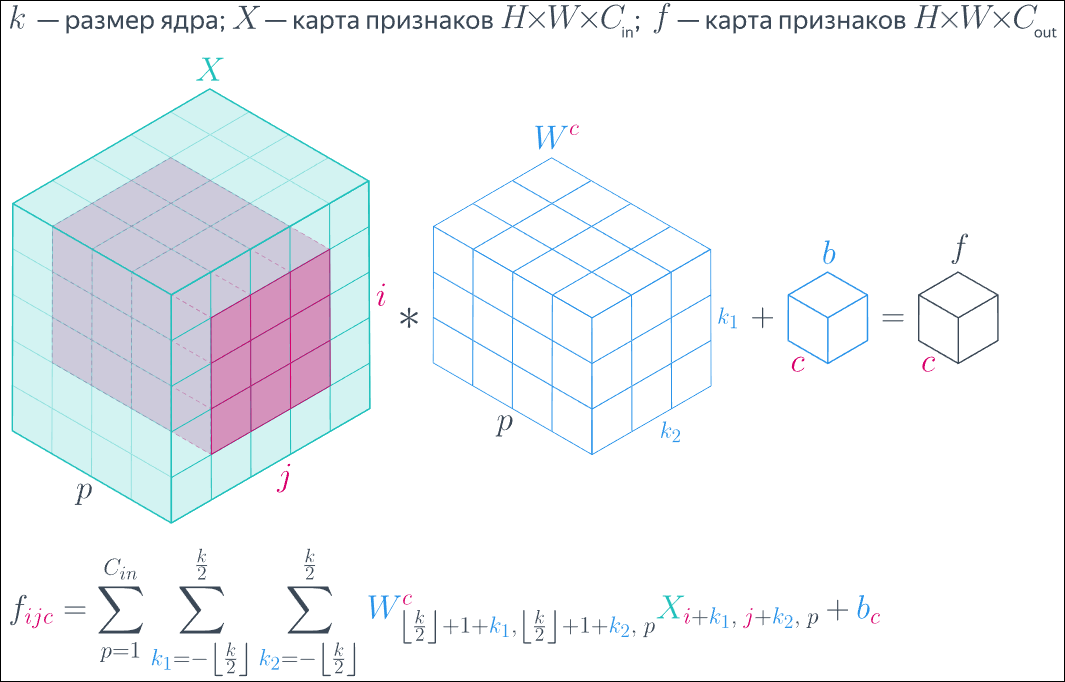
\includegraphics[width=0.9\linewidth]{img/conv_formula.png}
    \end{figure}
\end{frame}

\begin{frame}{Пример свёрток}
    \begin{columns}
        \begin{column}{0.5\textwidth}
            \[
                B _1 = \frac {1} {9} \begin{pmatrix}
                    1 & 1 & 1\\
                    1 & 1 & 1\\
                    1 & 1 & 1\\
                \end{pmatrix}
            \]
            Усредняет все пиксели размывая изображение.
        \end{column}

        \begin{column}{0.6\textwidth}
            \[
                B _2 = \begin{pmatrix}
                    -1 & -1 & -1\\
                    -1 & 8 & -1\\
                    -1 & -1 & -1\\
                \end{pmatrix}
            \]
            Смысл: пиксели из однородных участков изображения слабеют, тогда как контрастные точки, напротив, усиливаются.
        \end{column}
    \end{columns}
    

    \begin{figure}
        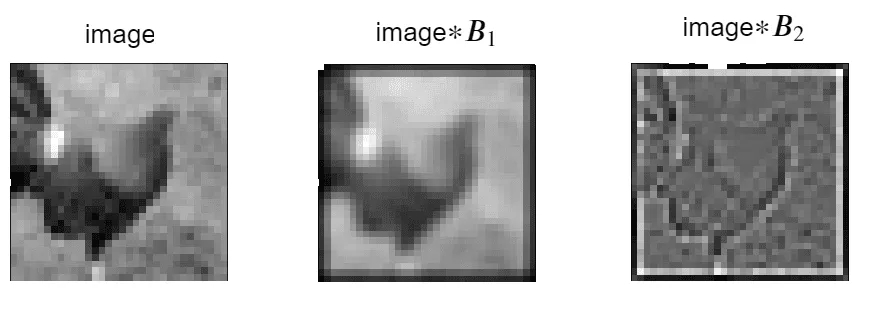
\includegraphics[width=\textwidth]{img/conv_example.jpg}
    \end{figure}
\end{frame}

\begin{frame}{Каналы и свёртки}
    \begin{itemize}
        \item Изначально в цветном изображении содержится три канала для каждого цвета;
        \item С каждой свёрткой мы уменьшаем размер изображения, но увеличиваем количество каналов;
        \item Каждый канал может отвечать за какой-то признак изображения (границы, определённые объекты и т.д.).
    \end{itemize}
    \begin{figure}
        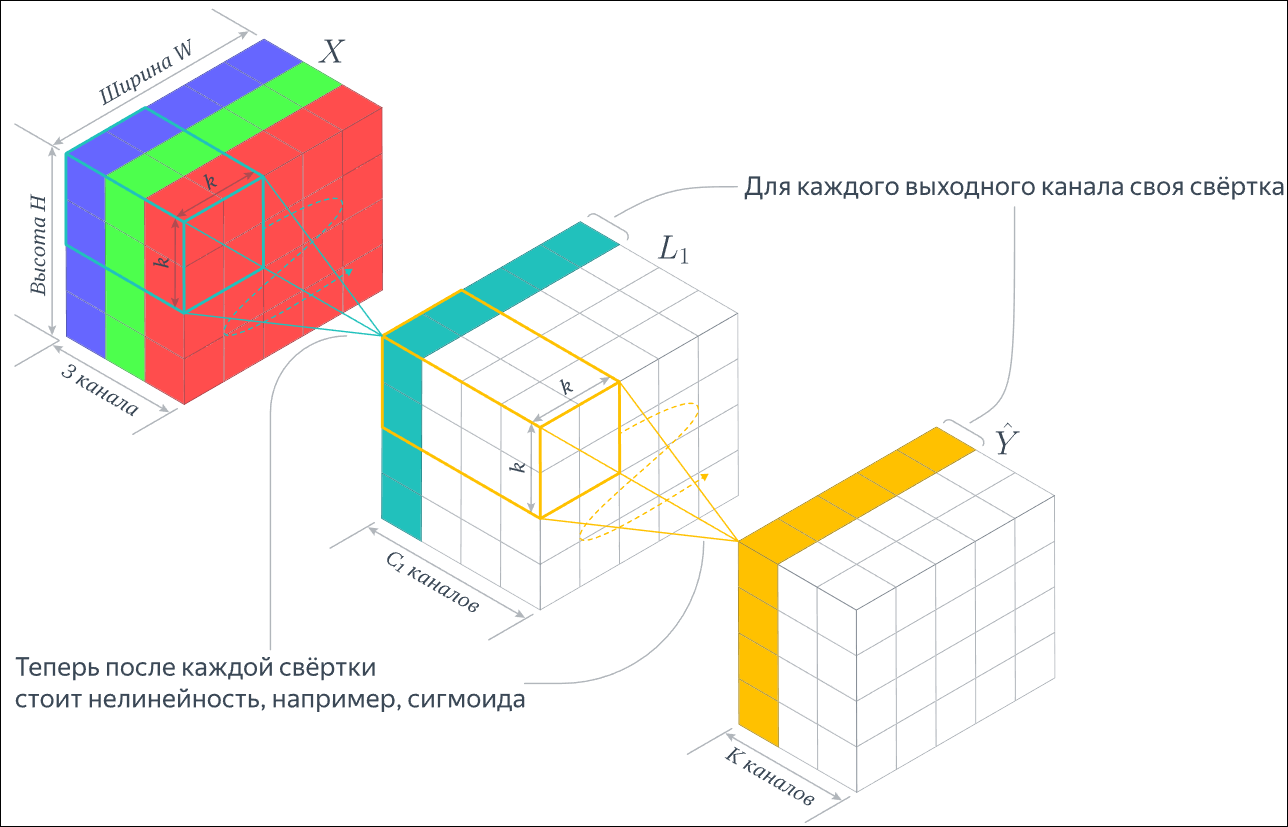
\includegraphics[width=0.8\textwidth]{img/canals.png}
    \end{figure}
\end{frame}

\begin{frame}{Pooling — уменьшение размерности}
    Хотим повысить количество каналов в каждой свёртке, чтобы выделять больше признаков. Проблема: слишком много параметров, решение: уменишить разрешение каждого канала.

    \begin{itemize}
        \item Max Pooling — берёт максимум из области;
        \item Average Pooling — усреднение значений;
        \item Снижает вычислительные затраты и переобучение.
    \end{itemize}
    \begin{figure}
        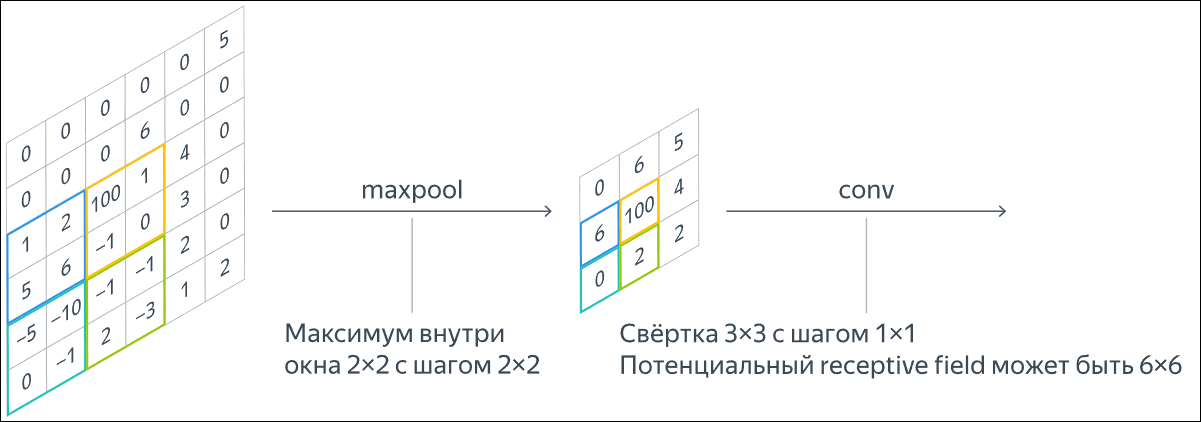
\includegraphics[width=\linewidth]{img/max_pooling.png}        
    \end{figure}
\end{frame}

\begin{frame}{Остальная часть}
    \begin{enumerate}
        \item После нескольких слоёв свёрток, ReLU и Max Pooling: либо тензор $1 \times 1 \times C$, либо $n \times m \times C$;
        \item В первом случае просто вытягиваем в вектор;
        \item Во втором: можем применить Global average pool --- пулинг по каналам;
        \item Далее применяется обычная полносвязная нейронная сеть.
    \end{enumerate}

    Для проблем с затуханием используем Residual connection.
\end{frame}

\begin{frame}{Задача классификации}
    Свёрточные нейронные сети хороши тем, что они end-to-end.

    \begin{itemize}
        \item Вход: изображение в виде двухмерных каналов цветов;
        \item Выход: метка класса (двуклассовая и многоклассовая классификация);
        \item Пример: распознавание животных, предметов, сцен и т.д.
    \end{itemize}

    \begin{figure}
        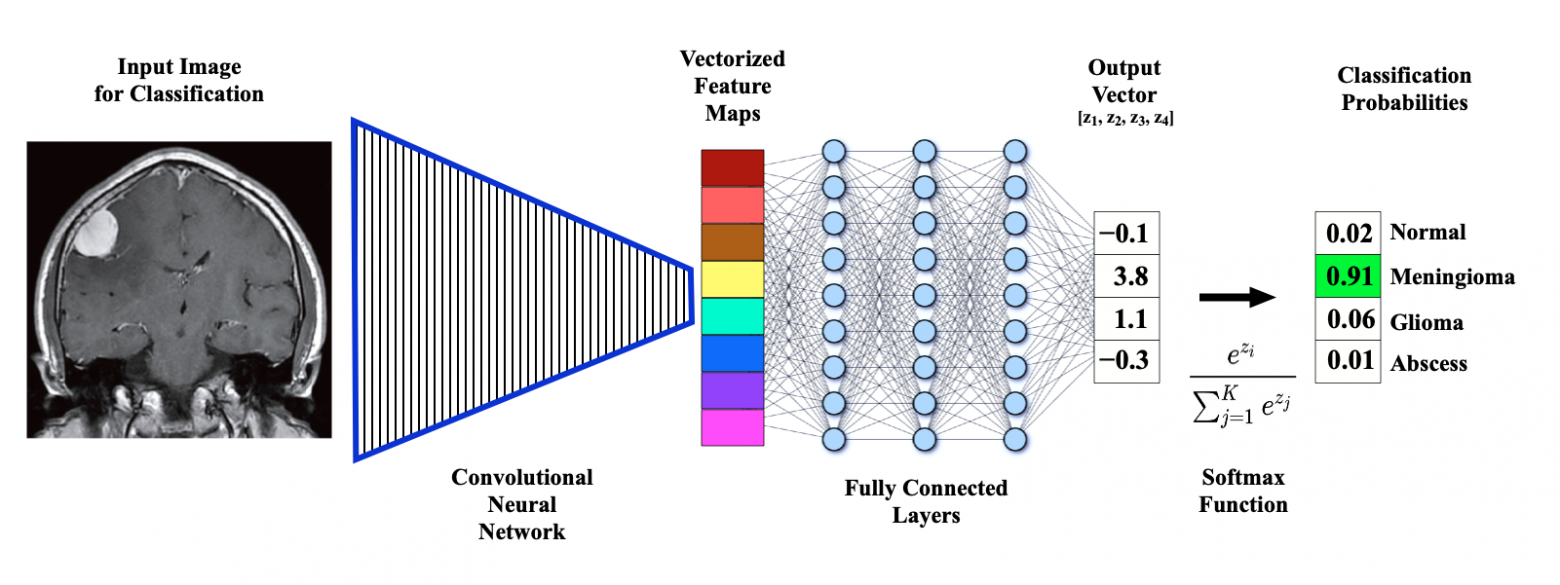
\includegraphics[width=\linewidth]{img/conv_classification.png}        
    \end{figure}
\end{frame}

\begin{frame}{Функция потерь и обучение}
    \begin{itemize}
        \item Для задачи классификации используется кросс-энтропия (Cross-Entropy Loss):
        \[
        \mathcal{L} = -\frac{1}{N} \sum_{i=1}^{N} \sum_{c=1}^{C} y_{i,c} \log(\hat{y}_{i,c})
        \]
        где $N$ — размер батча, $C$ — число классов, $y_{i,c} \in \{0,1\}$ — истинная метка (one-hot), $\hat{y}_{i,c}$ — вероятность, выданная softmax:
        \[
            \hat{y}_{i,c} = \frac{e^{z_{i,c}}}{\sum_{k=1}^{C} e^{z_{i,k}}}
        \]
        \item Используемые оптимизаторы: SGD, Adam
        \item Backpropagation.
        \[
            \frac{\partial \mathcal{L}}{\partial \theta} = \frac{\partial \mathcal{L}}{\partial \hat{y}} 
            \cdot \frac{\partial \hat{y}}{\partial z} 
            \cdot \frac{\partial z}{\partial \theta}
        \]
        — вычисляется градиент по параметрам сети.
    \end{itemize}
\end{frame}

\begin{frame}{Backpropagation в свёрточном слое}
    Обратный проход в свёрточном слое имеет несколько иную форму.

    \textit{Градиент по входу:}
    \[
    \frac{\partial \mathcal{L}}{\partial x _{i, j, c}} 
    = \sum _{k = 0} ^{C _{out} - 1} \sum _{m = 0} ^{M - 1} \sum _{n = 0} ^{N - 1} \frac{\partial \mathcal{L}}{\partial z _{i - m, j - n, k}} w _{m, n, c, k},
    \]
    --- это свёртка ошибки с перевёрнутым фильтром. $z _{i, j, k}$ --- значения следующего слоя.

    \textit{Градиент по весам:}
    \[
    \frac{\partial \mathcal{L}}{\partial w _{m, n, c, k}} 
    = \sum _{i, j} x _{i + m, j+n, c} \frac{\partial \mathcal{L}}{\partial z _{i, j, k}}.
    \]
    Вес обновляется пропорционально корреляции входа и ошибки

    \textit{Градиент по смещению:}
    \[
    \frac{\partial \mathcal{L}}{\partial b _k} 
    = \sum _{i, j} \frac{\partial \mathcal{L}}{\partial z _{i, j, k}}.
    \]
\end{frame}

\begin{frame}{Популярные архитектуры для классификации}
    \begin{itemize}
        \item LeNet (1998) (7 слоёв) --- первая свёрточная нейронная сеть, показавшая SOTA результаты на MNIST. Cвёрточные слои с ядром 5x5. Активация --- tanh, вместо max-pool --- average;
        \item AlexNet (2012) (11 слоёв) --- первая CNN, взявшая imagenet. ReLU вместо сигмоид, max-pool вместо average. Обучение на двух GPU;
        \item VGGNet (2014) (19 слоёв) --- ввели стандарт свёрток $3 \times 3$ и последовательное выполнение их с нелинейностями;
        \item ResNet (2015) (152 слоя) --- нынешний baseline, ввели skip connections и свёртки $1 \times 1$.
    \end{itemize}
    \begin{figure}
        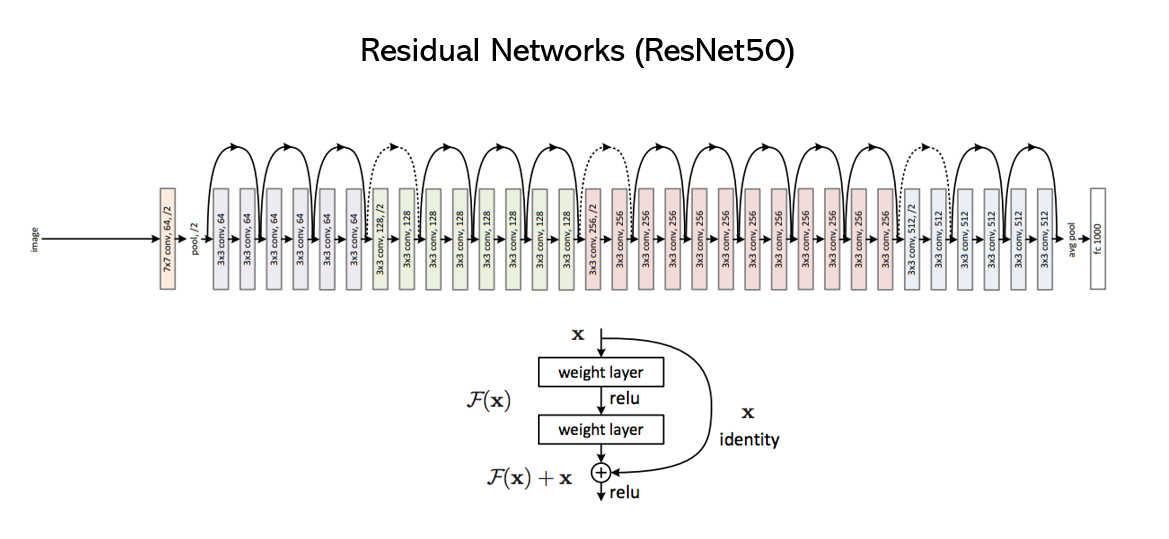
\includegraphics[width=\linewidth]{img/resnet.png}    
    \end{figure}
\end{frame}

\begin{frame}{Что такое сегментация}
    \textbf{Задача}: разделить изображение на осмысленные области (сегменты), соответствующие различным объектам или частям сцены.

    \begin{itemize}
        \item Пиксельная классификация изображения;
        \item Цель: выделить объекты на уровне пикселей;
        \item Применения: медицина, автономные автомобили, спутниковые снимки.
    \end{itemize}
    \begin{figure}
        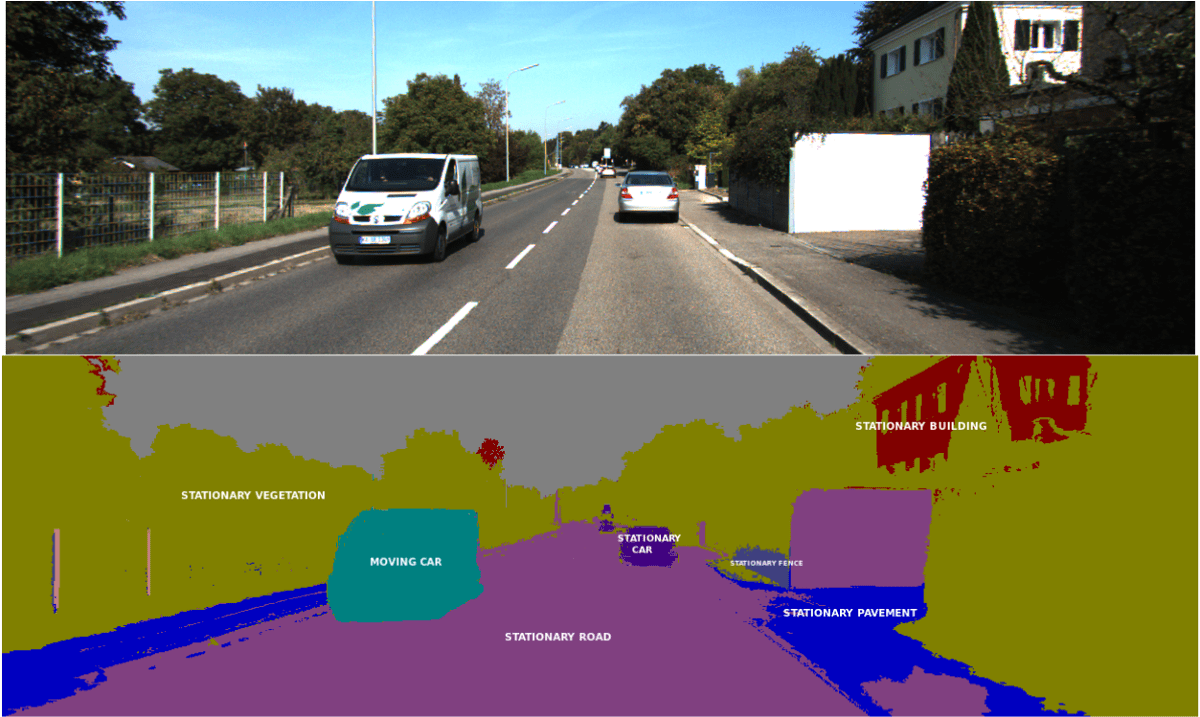
\includegraphics[width=0.8\linewidth]{img/segmentation.png}
    \end{figure}
\end{frame}

\begin{frame}{Формальное определение}
    Пусть у нас есть изображение:
    \[
        \mathbf{I} \in \mathbb{R} ^{H \times W \times C},
    \]
    где $H$ --- высота изображения, $W$ --- ширина, $C$ --- число каналов ($3$ в RGB).

    Задача сегментации --- найти отображение:
    \[
        f _\theta: \mathbb{R} ^{H \times W \times C} \to \{1, \dots, K\} ^{H \times W},
    \]
    где $K$ --- количество классов, а $f _\theta$ --- обучаемая модель, которая выдаёт карту классов для каждого пикселя.
\end{frame}

\begin{frame}{Виды сегментации}
    \begin{figure}
        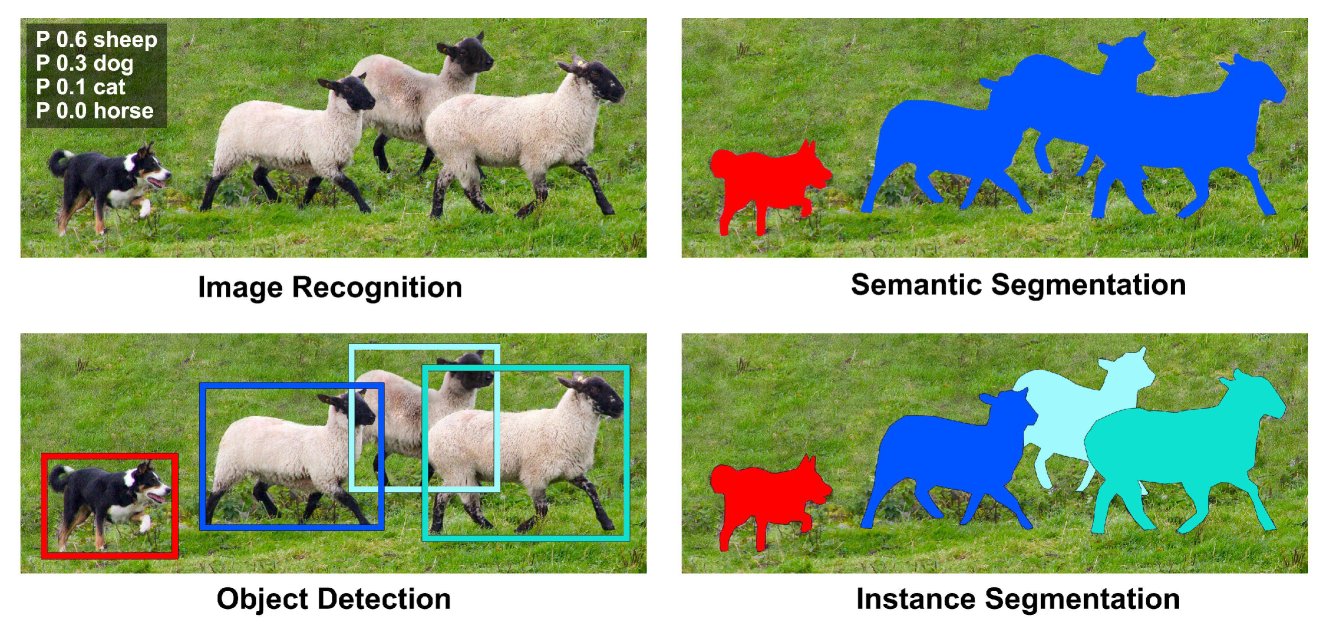
\includegraphics[width=0.7\linewidth]{img/segmentation_kind.png}        
    \end{figure}
    \begin{itemize}
        \item Семантическая сегментация --- классифицирует каждый пиксель по классу, не различая экземпляры (все кошки = один класс);
        \item Инстанс-сегментация --- различает отдельные экземпляры объектов одного класса (каждая кошка — отдельный объект);
        \item Паноптическая сегментация --- объединяет семантическую и инстанс-сегментацию (сцена со всеми типами объектов).
    \end{itemize}
\end{frame}

\begin{frame}{U-Net (2015)}
    \begin{itemize}
        \item Симметричная encoder-decoder архитектура, decoder использует транспонированные свёртки (upsampling);
        \item Skip-соединения между слоями (копирует признаки с энкодера и объединяет с декодером);
        \item Широко применяется в медицине.
    \end{itemize}

    \begin{figure}
        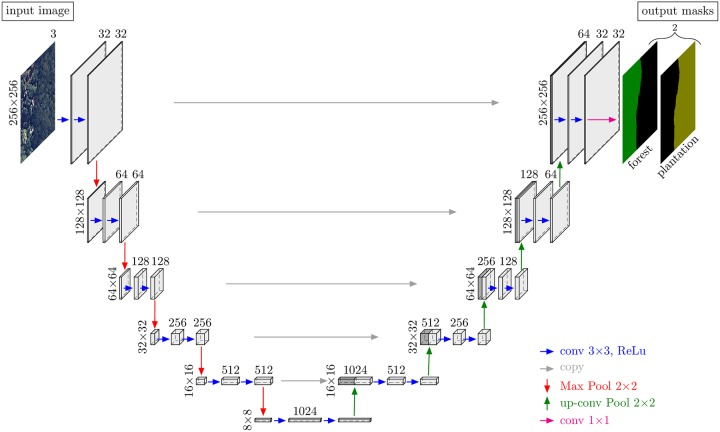
\includegraphics[width=0.8\linewidth]{img/u_net.jpg}    
    \end{figure}
\end{frame}

\begin{frame}{SegNet (2016)}
    \begin{figure}
        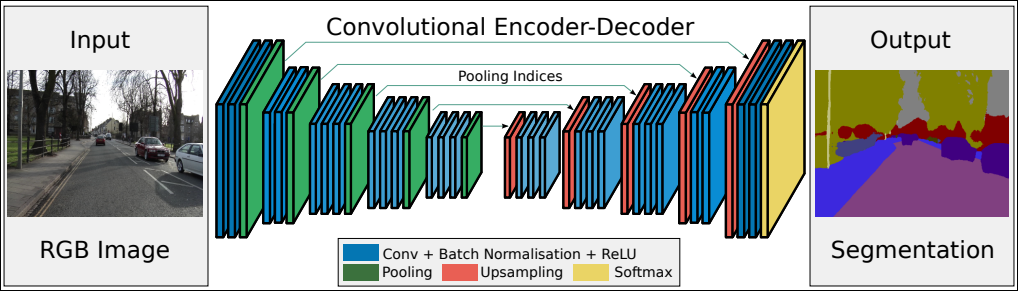
\includegraphics[width=\linewidth]{img/segnet.png}
    \end{figure}

    \begin{itemize}
        \item Использует индексы max pooling для восстановления формы;
        \item Нет skip-соединений, меньше параметров;
        \item Подходит для сегментации сцен в реальном времени.
    \end{itemize}
\end{frame}

\begin{frame}{DeepLab (v1–v3+) (2017–2018)}
    \begin{figure}
        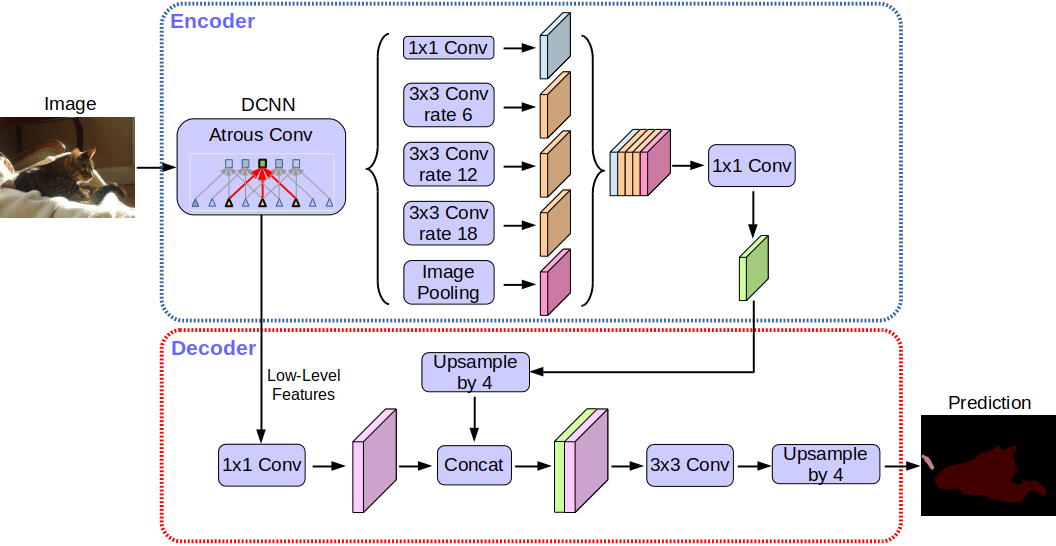
\includegraphics[width=\linewidth]{img/deeplab.png}
    \end{figure}

    \begin{itemize}
        \item Использует dilated convolutions
        \item Применяет CRF для уточнения границ объектов
        \item Высокая точность на сложных сценах
    \end{itemize}
\end{frame}

\begin{frame}{Метрики оценки в сегментации}
    \begin{enumerate}
        \item Стандартные оценки для классификации: accuracy, precision, recall, f1 и т.д. Здесь TP --- пиксели, правильно отнесённые к классу объекта, TN --- пиксели фона, правильно распознаные, FP --- пиксели фона, ошибочно отнесённые к объекту, FN --- пиксели объекта, пропущенные моделью.
        \item \textbf{Intersection over Union (IoU)} --- пересечение предсказанных и истинных областей:
        \[
            \text{IoU} = \frac{TP}{TP + FP + FN}, \quad
            \text{mIoU} = \frac{1}{K} \sum_{k=1}^{K} \text{IoU}_k
        \]
        \item \textbf{Dice Coefficient} используется для несбалансированных данных:
        \[
            \text{Dice} = \frac {2TP} {2TP + FP + FN}, \quad
            \text{Dice Loss} = 1 - \text{Dice}
        \]
    \end{enumerate}
\end{frame}

\end{document}